\documentclass{beamer}
\usetheme{Warsaw}
\usepackage{graphicx}
\useoutertheme{miniframes}

% Datos
\title{Event Driven Molecular Dynamics}
\author{Grupo 5}
\institute{ITBA}
\date{} % sin fecha
\setbeamertemplate{headline}[miniframes theme]
% Numerar diapositivas
\setbeamertemplate{footline}[frame number]

\begin{document}

% Portada
\begin{frame}
  \titlepage
  \begin{center}
      \small INTEGRANTES: MARTINA SCHVARTZ TALLONE, PATRICK LUCA TORLASCHI y SERGIO SMIRNOFF
  \end{center}
\end{frame}

% Introducción
\section{Introducción}
\subsection{Sistema Real}
\begin{frame}{Gas ideal, sistema de partículas rígidas por eventos}
  \textbf{Trayectoria recta, colisiones elásticas y sin gravedad}
  \vspace{0.5cm}
  \begin{itemize}
    % Descripción del sistema real.
    \item N partículas rígidas en movimiento.
    \item Cada partícula con su movimiento, posición, radio y masa.
    \item Viajan sin fuerzas externas.
    \item Colisiones elásticas entre partículas.
    \item Simulación de un sistema de eventos.
  \end{itemize}
  % imagen del sistema de eventos
  \begin{center}
    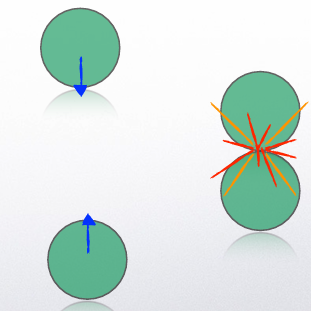
\includegraphics[width=0.3\linewidth]{photoMaterial/eventos_sistema_real.png}
  \end{center}
\end{frame}

\subsection{Modelo Matemático}
\begin{frame}{Modelo Matemático}
  \begin{itemize}
    \item Vuelo libre de las N partículas en un espacio 2D:
    \begin{itemize}
      \item $x_i(t) = x_i(0) + v_{x_i} t$
      \item $y_i(t) = y_i(0) + v_{y_i} t$
    \end{itemize}
    \item Cálculo de tiempo de colisión contra paredes:
    \begin{itemize}
      \item $t_{c} = \infty$ si $dv \cdot dr \geqslant 0$,
      \item $t_{c} = \infty$ si $d < 0$, siendo: $d = (dv \cdot dr)^2 - (dv \cdot dv)\cdot(dr \cdot dr - \sigma^2 )$,
      \item $\sigma = r_i + r_j$
      \item Colisión con paredes espejan la velocidad en la normal de colisión.
    \end{itemize}
  \end{itemize}
\end{frame}

% Colisiones entre particulas, formulas
\begin{frame}{Modelo Matemático}
  \begin{itemize}
    \item Cálculo de impulso y velocidades post-colisión de partículas:
      \begin{itemize}
        \item $J_x = J*dx/\sigma$
        \item $J_y = J*dy/\sigma$
        \item $J = \dfrac{2 m_i m_j}{m_i + m_j} \cdot \dfrac{dv \cdot dr}{\sigma}$
        \item $vx_i^d = vx_i^a + J_x/m_i$
        \item $vy_i^d = vy_i^a + J_y/m_i$
        \item $vx_j^d = vx_j^a - J_x/m_j$
        \item $vy_j^d = vy_j^a - J_y/m_j$
      \end{itemize}
  \end{itemize}
\end{frame}

% Implementación
\section{Implementación}
\begin{frame}{Implementación}
  \begin{columns}
    \begin{column}{0.4\textwidth}
      {\scriptsize
        \begin{center}
          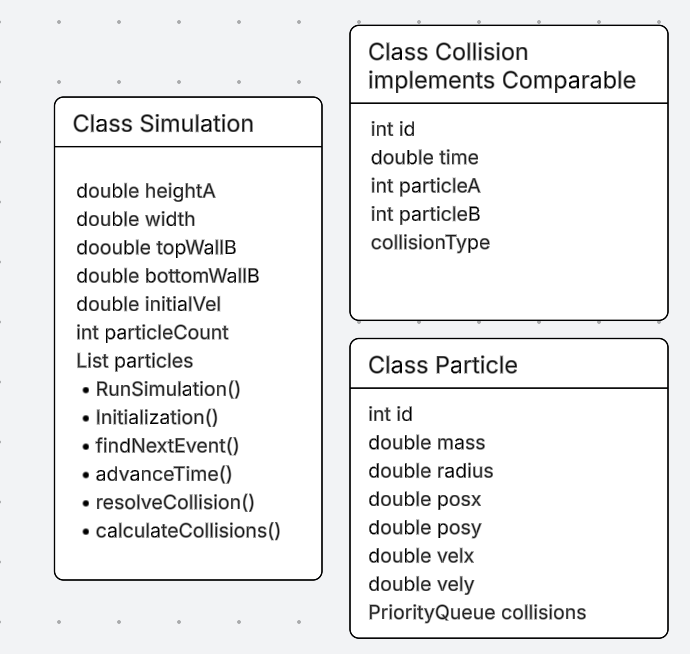
\includegraphics[width=0.9\linewidth]{photoMaterial/uml.png}
        \end{center}
      }
    \end{column}
    \begin{column}{0.6\textwidth}
      {\scriptsize
        \textbf{Estructura del código y elementos importantes:}
        \begin{itemize}
          \item \texttt{Main(maxIter, nombreArchivo, L)}
          \item \texttt{runSimulation} $\rightarrow$ realiza las iteraciones separadas en:
          \begin{itemize}
            \scriptsize{
            \item \texttt{initialization()} $\rightarrow$ Se inicializan las partículas.
            \item \texttt{inicialCollisions()} $\rightarrow$ Se calculan las colisiones iniciales.
            \item \texttt{findNextEvent()} $\rightarrow$ Encuentra el próximo evento.
            \item \texttt{advanceTime()} $\rightarrow$ Avanza el tiempo y actualiza las posiciones de las partículas.
            \item \texttt{resolveCollision()} $\rightarrow$ Procesa el evento.
            }
          \end{itemize}
          \item Clase \texttt{Particle}
          \item Clase \texttt{Colisions}
        \end{itemize}
      }
    \end{column}
  \end{columns}
\end{frame}


\begin{frame}{Implementación de vértices}
  % Consultar martina
  \begin{itemize}
    \item Tiempo a colisión con pared horizontal = tiempo a colisión con pared vertical $\leftarrow$ vértice.
    \item Se tienen 1 partícula en cada vértice.
    \item Características:
      \begin{itemize}
        \item Radio = 0.
        \item Masa = $\infty$.
      \end{itemize}
    \item Espejan las velocidades en los distintos choques.
    \item No se mueven.
  \end{itemize}
\end{frame}

% Simulaciones

\begin{frame}{Geometría del sistema y parámetros de simulación}
  \scriptsize
  \begin{columns}
    \begin{column}{0.5\textwidth}
      \textbf{Geometría:}
      \begin{itemize}
        \item Dos cajas A y B, conectadas por una abertura de tamaño $L$.
        \item Las partículas se distribuyen uniformemente en la caja A al inicio de la simulación sin superponerse.
      \end{itemize}
      \vspace{0.2cm}
      \begin{center}
        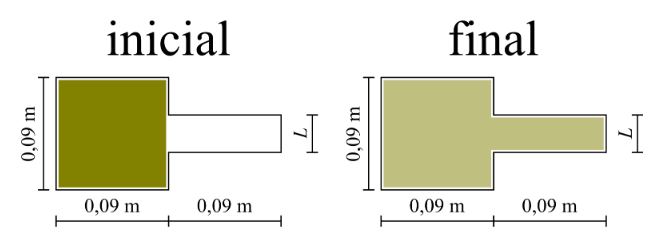
\includegraphics[width=0.85\linewidth]{photoMaterial/geometria.jpg}
      \end{center}
    \end{column}
    \begin{column}{0.5\textwidth}
      \textbf{Constantes:}
      \begin{itemize}
        \item Número de partículas: 250.
        \item Dimensiones caja A: \textit{0.09} m $\times$ \textit{0.09} m.
        \item Dimensiones caja B: \textit{0.09} m ancho.
        \item Radio de partículas: \textit{0.0015} m.
        \item Masa de partículas: \textit{1} kg.
        \item Velocidad inicial: \textit{0.01} m/s.
      \end{itemize}
      \vspace{0.2cm}
      \textbf{Variables:}
      \begin{itemize}
        \item $L \in \{ \textit{0.09}, \textit{0.07}, \textit{0.05}, \textit{0.03} \}$
      \end{itemize}
    \end{column}
  \end{columns}
\end{frame}

\begin{frame}{Definición matemática de observables}
  \textbf{Observables}
  \begin{itemize}
    \item Presión en las cajas A y B.
    \item Calculándolas como la suma de los impulsos por colisiones contra la pared por unidad de tiempo.
    \item Se obtiene con la fórmula: $P = \frac{1}{A} \sum J_i$ siendo A el área de la pared y $J_i$ el impulso de cada colisión.
    \item $J_i = 2 * v_n$ siendo $v_n$ la velocidad de la partícula.
    \item Coeficiente cuadrático medio: $<z^2> = 2Dt$
  \end{itemize}
\end{frame}

% Resultados
\section{Resultados}
\subsection{Animaciones}
\begin{frame}{Animaciones}
  % Aquí va la imagen de un frame representativo
  \includegraphics[width=0.7\linewidth]{ejemplo.png}
  \vspace{0.3cm}
  \footnotesize Link al video: \url{https://youtube.com/...}
\end{frame}

\begin{frame}{Evolución temporal del observable}
  \begin{columns}
    \begin{column}{0.5\textwidth}
      \tiny \textit{Presión en función del tiempo para $L = \textit{0.09}$ m.}
      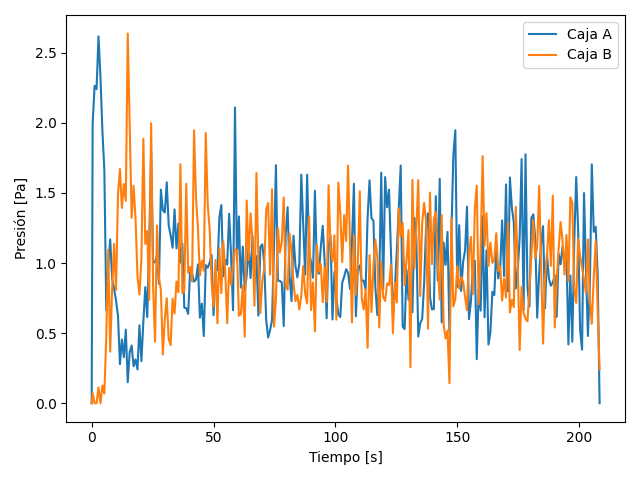
\includegraphics[width=\linewidth]{photoMaterial/pvt_09.png}
    \end{column}
    \begin{column}{0.5\textwidth}
      \tiny \textit{Presión en función del tiempo para $L = \textit{0.07}$ m.}
      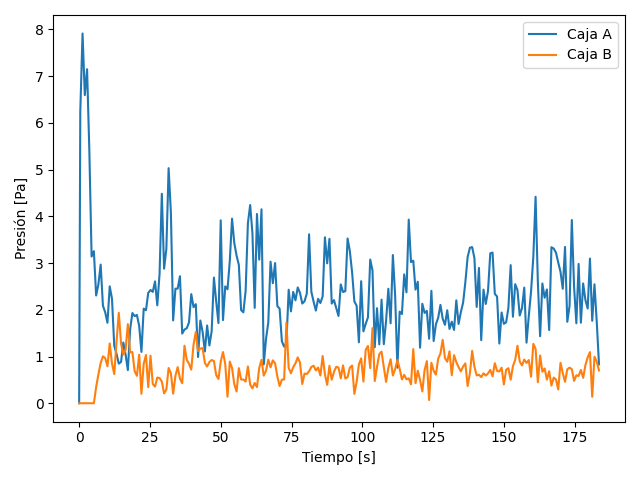
\includegraphics[width=\linewidth]{photoMaterial/pvt_07.png}
    \end{column}
    \end{columns}
    \tiny Podemos tomar estacionario a partir de los 20 segundos.
    \tiny Con: N = \textit{250}, r = \textit{0.0015} m, m = \textit{1} kg.
\end{frame}
\subsection{Input vs Observable}
\begin{frame}{Evolución temporal del observable}
  \begin{columns}
    \begin{column}{0.5\textwidth}
      \scriptsize \textit{Presión en función del tiempo para $L = \textit{0.05}$ m.}
      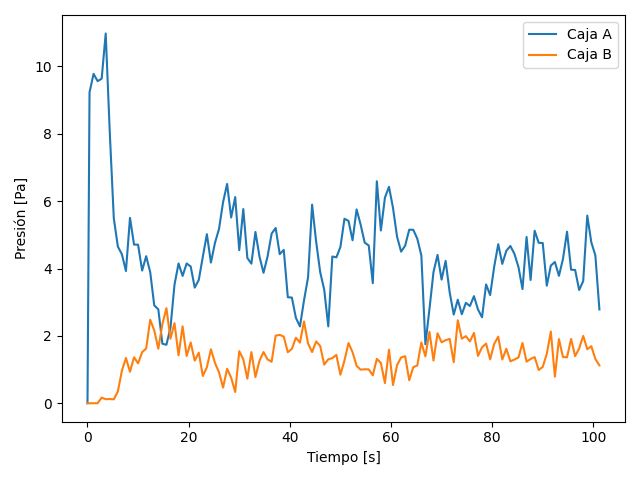
\includegraphics[width=\linewidth]{photoMaterial/pvt_05.png}
    \end{column}
    \begin{column}{0.5\textwidth}
      \scriptsize \textit{Presión en función del tiempo para $L = \textit{0.03}$ m.}
      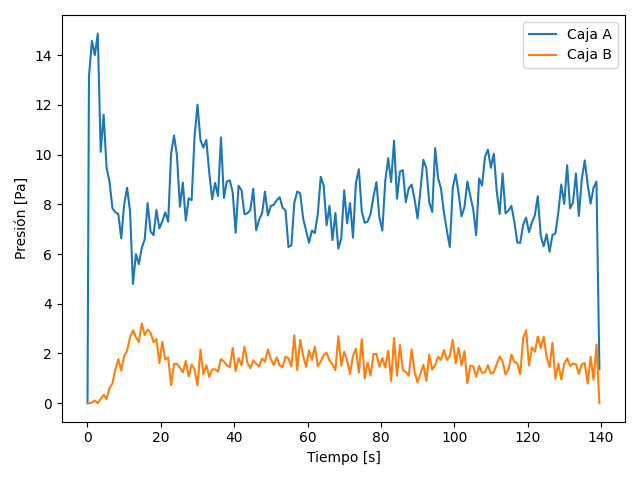
\includegraphics[width=\linewidth]{photoMaterial/pvt_03.png}
    \end{column}
  \end{columns}
  \tiny Podemos tomar estacionario a partir de los 20 segundos.
  \tiny Con: N = \textit{250}, r = \textit{0.0015} m, m = \textit{1} kg.
\end{frame}

\begin{frame}{Primer estudio: Presión vs $A^{-1}$}
  \begin{columns}
    \begin{column}{0.40\textwidth}
      \scriptsize \text{Input}
      \begin{itemize}
        \item $L \in \{ \textit{0.09}, \textit{0.007}, \textit{0.05}, \textit{0.03} \}$ m.
        \item $v_o$ = \textit{0.01} m/s.
        \item $r$ = \textit{0.0015} m.
        \item $m$ = \textit{1} kg.
        \item $N$ = 250.
      \end{itemize}
    \end{column}
    \begin{column}{0.60\textwidth}
      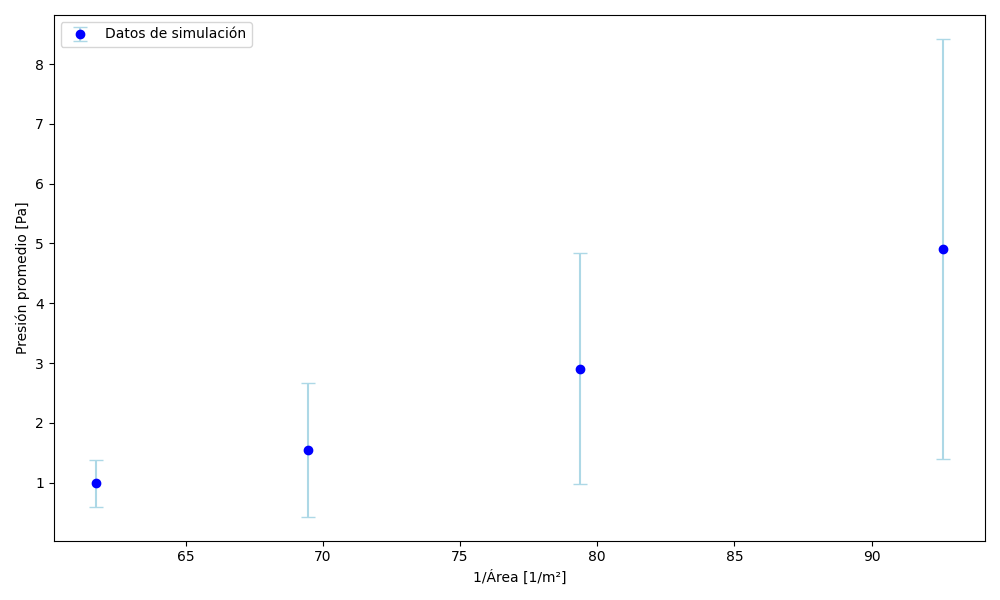
\includegraphics[width=1\linewidth]{photoMaterial/Presion_vs_area.png} % meter el de area real
      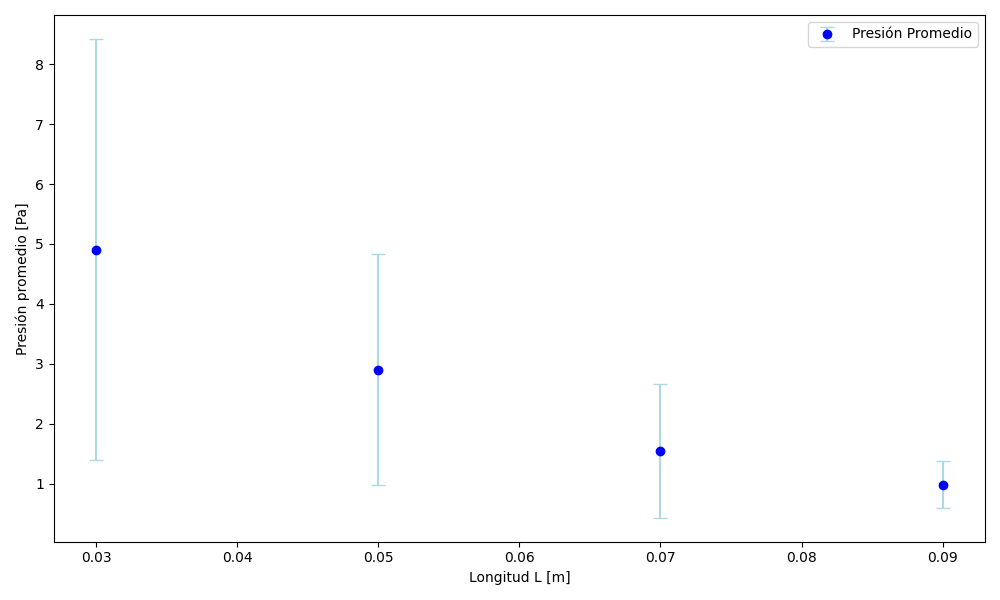
\includegraphics[width=1\linewidth]{photoMaterial/Presion_vs_L.png}
    \end{column}
  \end{columns}
\end{frame}

\begin{frame}{Primer estudio: Presión vs $A^{-1}$}
  \begin{columns}
    \begin{column}{0.40\textwidth}
      \scriptsize \text{Input}
      \begin{itemize}
        \item $L \in \{ \textit{0.09}, \textit{0.007}, \textit{0.05}, \textit{0.03} \}$ m.
        \item $v_o$ = \textit{0.01} m/s.
        \item $r$ = \textit{0.0015} m.
        \item $m$ = \textit{1} kg.
        \item $N$ = 250.
      \end{itemize}
    \end{column}
    \begin{column}{0.60\textwidth}
      %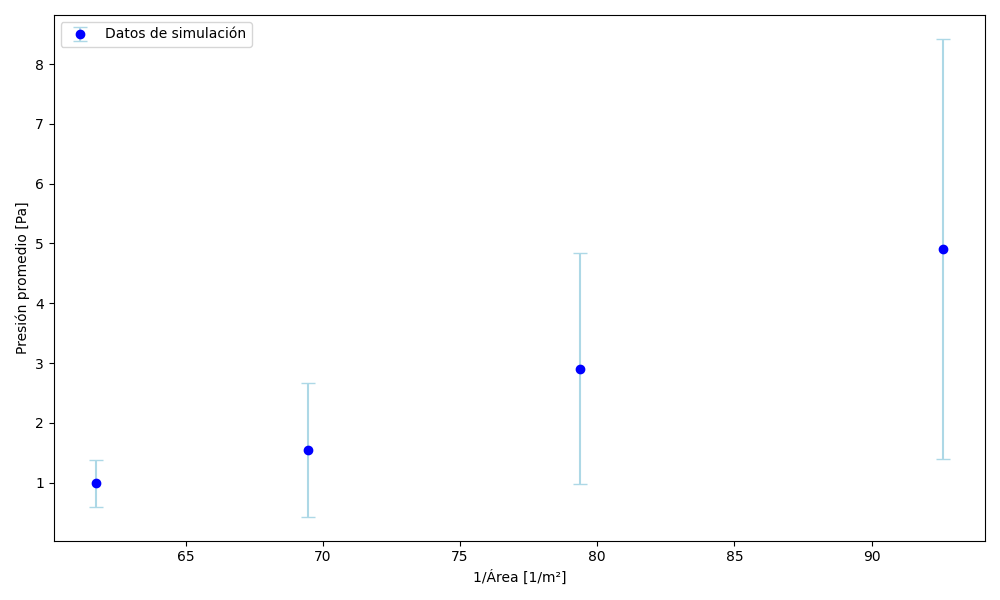
\includegraphics[width=0.75\linewidth]{photoMaterial/Presion_vs_area.png} ver si meterlo o no
      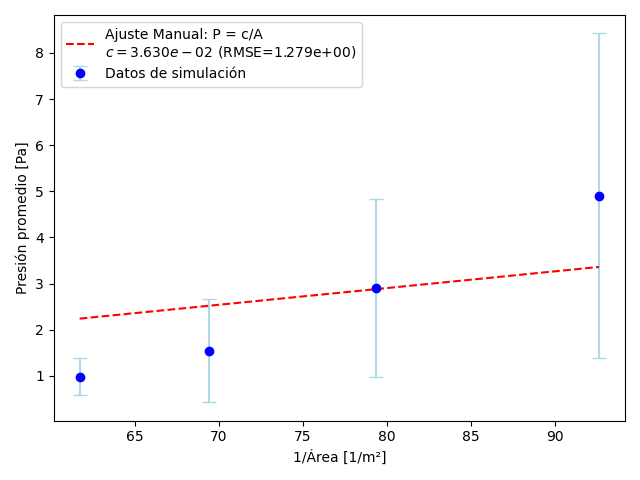
\includegraphics[width=1\linewidth]{photoMaterial/Presion_vs_area_ajuste.png}
    \end{column}
  \end{columns}
\end{frame}

\subsection{Segundo estudio: Coeficiente de difusión}
\begin{frame}{Coeficiente de difusión}
  \tiny \text{Input:} $L$ = \textit{0.09} m -- $v_o$ = \textit{0.01} m/s -- $r$ = \textit{0.0015} m -- $m$ = \textit{1} kg -- $N$ = 250.
  \begin{columns}
    \begin{column}{0.50\textwidth}
      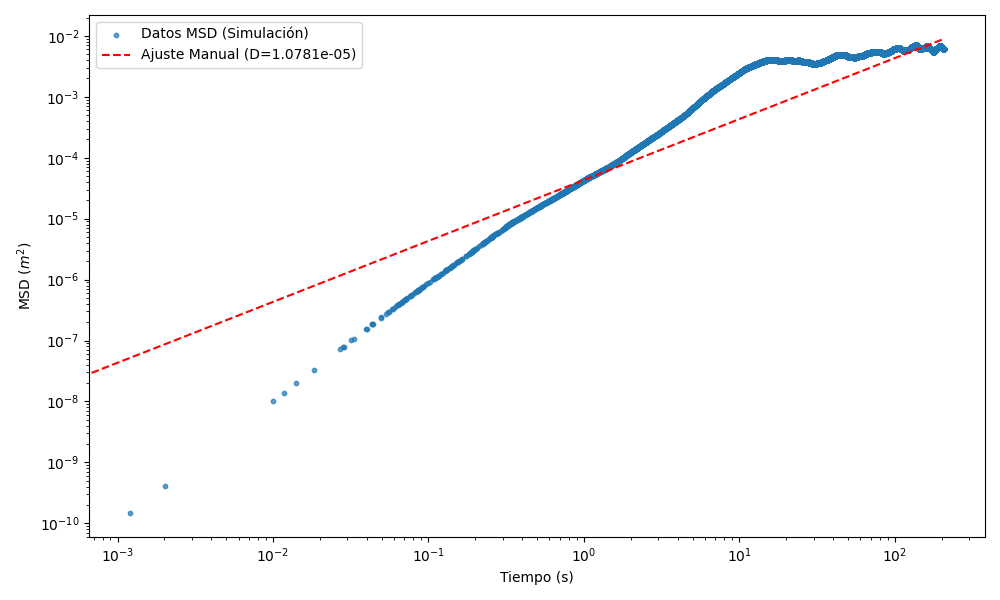
\includegraphics[width=1.10\linewidth]{photoMaterial/MSD_09.png}
    \end{column}
    \begin{column}{0.50\textwidth}
      %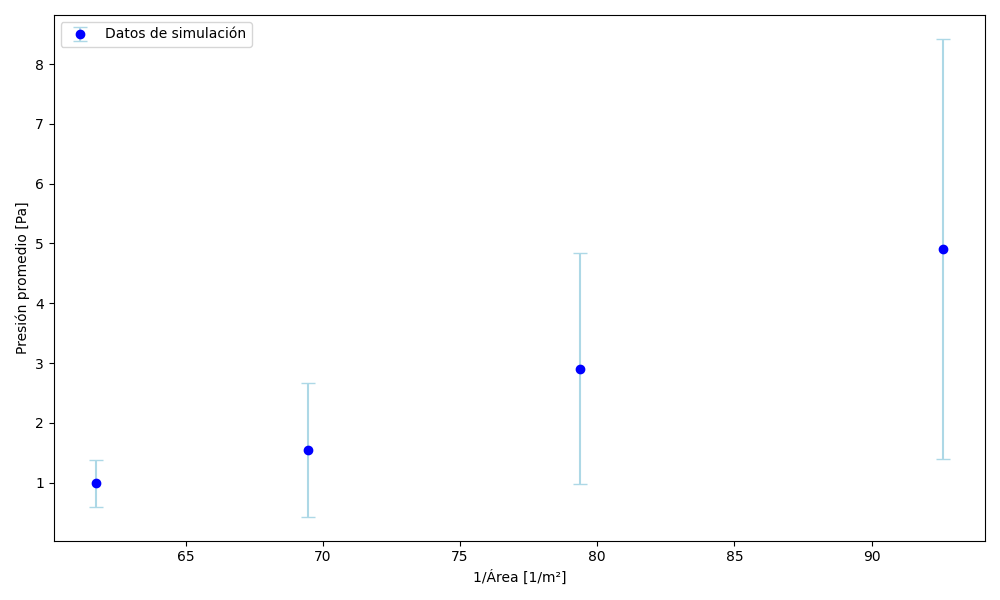
\includegraphics[width=0.75\linewidth]{photoMaterial/Presion_vs_area.png} ver si meterlo o no
      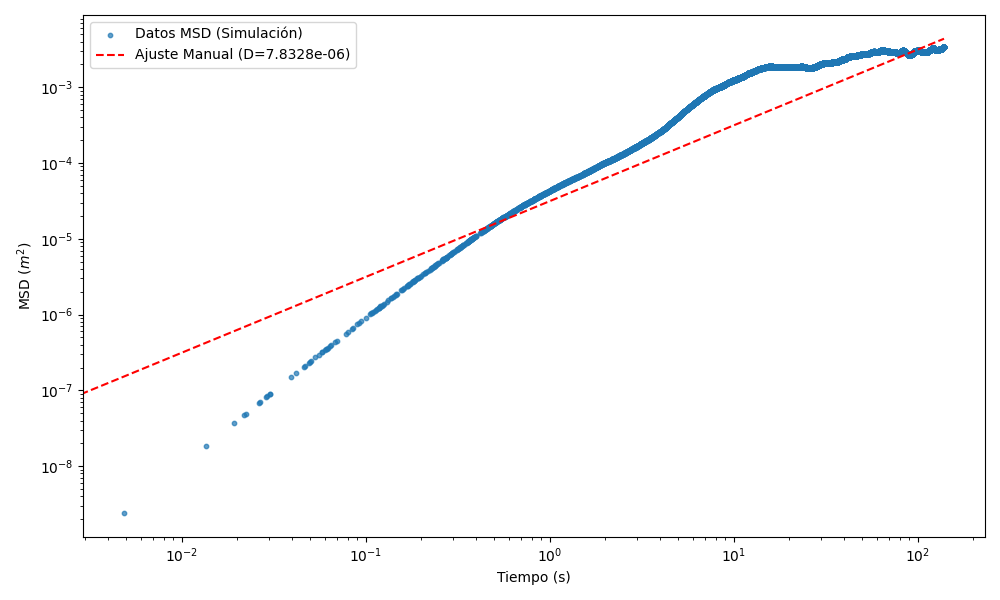
\includegraphics[width=1.10\linewidth]{photoMaterial/MSD_03.png}
    \end{column}
  \end{columns}
\end{frame}

% Conclusiones
\section{Conclusiones}
\begin{frame}{Conclusiones}
  \textbf{Primer estudio: Presión vs $A^{-1}$}
  \begin{itemize}
    \item Cuanta mayor área, menor es la presión.
    \item Luego de 20 segundos, todas las presiones entran en un régimen estacionario.
    \item NO se cumple la ley de los gases ideales ya que P no es cte.
  \end{itemize}
  \textbf{Segundo estudio: Coeficiente de difusión}
  \begin{itemize}
    \item Falta este análisis.
  \end{itemize}
\end{frame}

% Cierre
\begin{frame}{}
  \centering
  \Huge ¡Gracias por su atención!
\end{frame}

\end{document}

